\documentclass[11pt]{informatics-report}
\usepackage[utf8]{inputenc}
\usepackage[backend=biber, sorting=none]{biblatex}
\usepackage[nottoc,numbib]{tocbibind}
\usepackage{textgreek}
\usepackage{graphicx}
\usepackage{pdfpages}
\graphicspath{ {./images/} }
\addbibresource{bibliography.bib}
\title{Agent-based simulation of bicycle theft in London}
\author{Emily Liu}
\studentID{1744993}
\supervisor{Dr Simon Miles}

\date{May 6, 2020}

\abstractFile{FrontMatter/abstract.tex}
\ackFile{FrontMatter/acknowledgements.tex} %Remove line if you do not want acknowledgements

\begin{document}
\createFrontMatter
\tableofcontents

\chapter{Introduction}
Exercise is generally accepted to have a positive effect on cardiovascular health, advice from the NHS states that "regular cycling can reduce the risk of chronic illnesses such as heart disease and stroke"\cite{nhs}. One of the easiest ways to fit cycling into your routine is to use it as a means of transport. Cycling in London has grown year on year with numbers doubling in the capital since 2000 \cite{latransport}, and between 2012 and 2017 featuring an overall 24 per cent increase  \cite{actionplan}. In 2018 Transport for London (TfL) estimated that 730,000 trips are made a day by bicycle \cite{tfl}. \par
Bicycle theft is viewed as a low risk, high reward crime with many 'CRAVED' features, for example they are widely available, often expensive, easy to use and there are numerous channels through which they can be sold \cite{ucl}. CRAVED features are those that are Concealable, Removable, Available, Valuable, Enjoyable and Disposable \cite{craved}. \par

In a report commissioned by the Mayor of London, it was noted that people are generally put off cycling due to the fear of having their bicycle stolen \cite{actionplan}. To reduce the number of bicycle thefts, a possible intervention could be to plant 'bait bikes' designed to detect thieves in the act. However interventions like this are often expensive and the effectiveness is not known prior to commencement. \par

An agent-based model (ABM) is a computational model where actions and interactions of agents can be simulated, this provides a unique way of simulating hypothesised societal effects. The use of ABMs to model bicycle theft will allow different crime deterrent policies to be tested prior to implementation in the real world to understand potential effects.

\section{Project aims}
The fundamental objective of the project is to develop a simulation of bicycle theft using ABM, focussing on interventions to deter offenders committing theft of bicycles. \par
Moreover, the ABM will act as a useful tool to evaluate the effectiveness of any interventions prior to real world utilization. An agent's decisions will be strongly influenced by its spacial and social network, a thief is more likely to offend if others within their network also commit theft. 
\chapter{Background}

\section{Cycling in  London and bicycle theft}
London has seen a 'cycle revolution' since the Livingston era in 2000. Cycling has been widely recognised as providing benefits to the health of individuals and to society, as a sustainable mode of transport in urban environments. The creation of Cycleways -routes that link communities, businesses and destinations across London in one cycle network \cite{cycleway} - has made cycling safer, encouraging more people to cycle. According to estimates by TfL in 2018 730,000 trips are made by bicycle daily in London \cite{tfl} compared with only 270,000 trips in 2000 \cite{tfl2}. With the Mayor of London's Cycling action plan, which is primarily focused on expanding cycle routes to connect more people, this number is only going to continue growing. \par

In recent times, with the declared climate emergency and increased congestion within London the Mayor's plan is to increase the already growing number of journeys made by bicycle to 1.3 million every day by 2024, to be supported by £2.3bn funding\cite{actionplan} in the hopes of transforming London into a cycling city.\par

Between September 2016 and September 2019 there were 60,552 reported bicycle thefts within the the Metropolitan Police's jurisdiction. It is important to note that the realistic number of bicycle thefts is most likely a lot higher, research has found that only one in every five bicycle theft is reported \cite{ucl}. It is clear that an intervention will be necessary sooner rather than later as the number of bicycles in London is projected to continually grow. With more bicycles on the streets of London, there is a greater opportunity for offenders to partake in bicycle theft. \par

Analysis of reported thefts has shown that bicycle theft continues to rise and this is not limited to London, it is throughout England and Wales, even while there is a decline in overall offending rate. The increase has been linked with the ease of liquidating bicycles whether that be whole or as parts and also it's high utility for door-to-door transportation. Between 2013 and 2016 figures show that the perpetrators of 96 percent of reported bicycle thefts in London were unidentified \cite{environment}. \par

\section{Criminology}
There have been several crime opportunity theories associated with theft, one of those being the Routine Activities theory (RCT) \cite{cohen} which focuses specifically on the characteristics of crime instead of the offenders. RCT is often used in urban settings, the theory states that for a crime to occur, three elements must be present: an available and suitable target; a motivated offender; and no authority figure to prevent the crime from happening \cite{rational}. It is through daily routine activity that the aforementioned elements interact and why places that attract high population present opportunities for crime \cite{sherman}. For instance, the large number of bicycles that are left near or at railway stations for hours at a time are bound to attract thieves because railways provide intermediate transportation for many cyclists. The idea is that if a bicycle is not protected enough, if it is worth the reward, crime will occur- if there is opportunity, there is crime. \par

Rational choice theory (RCT) describes humans as rational actors who calculate the rationality of committing crime using means and ends, costs and benefits \cite{cornishclarke}. Higher priced bicycles are more likely to be targeted than lower priced bicycles as a result of offenders selecting objects that maximise their expected utility. Sometimes theft does not take place even when offenders interact with the target, this is because the perceived risk is simply too high \cite{environment}. RCT aides situational crime prevention, specifically opportunity reducing measures that can be directed at opportunistic crime- in this case bicycle theft. \par


\section{Agent-based modelling}
An Agent-Based Model (ABM) is a computer based simulation which comprises of a collection of autonomous decision-making entities called agents, these agents are given rules for their interaction with other agents or entities within the confined environment which is being modelled. It is through these rules and interactions that patterns emerge \cite{abm}. Agents can represent individuals, groups or objects. Through the model iterations, each agent is able to assess its situation and make an informed decision as to its next steps via a set of probabilistic rules.\par

An ABM comprises of two parts,the first being the system and the component being the second- this being the environment and the agent. The relationship between the system and the component element is key to ABM's. The system defines the environment that the agents are bound by and interact within and also the properties for the whole model. Agents receive input from this environment and this in turn affects the way agents function in terms of their set of rules. With this, agents have the ability to gather information and perform actions in response to the the system's input. \par

It can be said that the environment and the agents operate on a need-to-know basis where the environment has no knowledge of specific agent behaviours and is not able to calculate the outcome of the model. The environment can however show the overall state of the system, this is by amassing individual agents' properties at a time tick in the model. Individual agents do not have knowledge of the whole system but instead rely on the local environment to make decisions by gathering information about the local environment and responding depending on their input, through interactions like this emergent phenomena can be captured. \par

The utilisation of agent-based modelling to crime is a relatively new concept, first appearing in the early to mid-2000s \cite{groff}. These models were initially used in formalizing theories and more recently used to predict crime in specific places and to understand patterns of crime for example in robbery. Within criminology, ABM's application to investigate situational crime prevention techniques has great potential. It could be used to provide 'what if' analyses which can include the effects that crime reduction plans might have before their implication. \cite{Malleson2014}. 

\subsubsection{Existing agent-based models in criminology}
ABMs have only recently began to be realised in criminology with early models being relatively simple and as a result, studies of direct relevant to crime deterrence are scarce. Some authors have implemented agent-based models of other crime types, for example cyber crime and pick-pocketing. The most relevant work is that of (Malleson et al, 2010)\cite{malleson2010} who build an agent-based model of burglary, specifically crime reduction through simulation using the PECS framework focusing on a behavioural model. This model purely focuses on offender behaviour and their need to commit burglary for financial gain.\par

In a report published in the Journal of Quantitative Criminology, it was concluded that at present, "the lack of model detail reported in publications make it difficult to assess where sufficient evidence exists to support the development of models" \cite{groff}. \par

The model proposed in this research will focus predominantly on the behaviour of victims and how victims can utilise preventative measures to reduce the chance of theft occurring through the opportunity theory framework. 

\subsection{Types of simulation systems for agent-based modelling}
%{talk about agent based modelling softwares, MASON, NetLogo, REPAST}

There are generally two types of simulation systems that can be used to develop agent-based models, these being either toolkits or software. Toolkits are modelling systems that provide a framework for the design of ABMs that provide libraries of software functionality consisting of pre-defined modules, routines and functions specifically designed for ABM. The use of toolkits can make it easier for modellers when faced with programming parts that are content-specific for example a Graphical User Interface and visualisation of the model. As the toolkits have been created and optimised by professional developers the reliability of the model and the efficiency of the algorithm is increased when thinking of the complex parts in models. \par 

However, there are limitations of using toolkits in the development of agent-based models. The modeller will be required to understand how to design and implement models in the toolkit, which can take a considerable amount of effort. Whilst most toolkits do provide demonstration models they can be difficult to understand and also difficult to apply to another purpose. Additional tools may be available from the wider user community but once again, the function may not be applicable for the chosen model purpose. Another issue is the lack of compatibility when dealing with model functions as there can be a lot of conflicts in the later stages of the development process. \par

As mentioned previously, software is also available for the development of agent-based models- software is useful for rapid development of prototype models. Modellers choosing to use software are typically restricted to the software's design framework, for example some software will have a limited environment to model within or limited number of agents available at any one time. Although there are drawbacks of using software other toolkits, ABM software is sufficient for the aims of the project as stipulated in 1.1 and is what will be focused upon in this paper. \par

\subsubsection{MASON}
MASON (Multi Agent Simulation Of Neighbourhood) was developed at George Mason University's Evolutionary Computation Laboratory with the Center for Social Complexity in 2003. MASON is rather complex in comparison with other available open-source software, it is suited for simulations that require long computations like multi-agent ABMs. Unfortunately technical documentation for MASON is limited and the user group in comparison with other software is somewhat limited. With the lack of debugging and lack of terminal window for users, it can be concluded that it is not user-friendly when compared with others and is most suitable for projects requiring fast computation.

\subsubsection{Repast}
Repast, the Recursive Porous Agent Simulation Toolkit, was originally developed at the University of Chicago but is now maintained by the Argonne National Laboratory. The tool originally catered for three programming languages from which models could be implemented: Java (RepastJ), Microsoft.Net(Repast.NET) and Python (RepastPy). This was all outmoded by Repast Simphony which provides all the functionality of previous Repast's but exclusively in Java. Although Repast is one of the fastest platforms currently available and feature advanced modelling capabilities, it is also one of the most complex mainly focused towards programming experts with a non user-friendly environment. 

\subsubsection{AgentSheets}
AgentSheets is a proprietary modelling system that allows individuals with limited prior programming experience to effortlessly develop agent-based models. The ease of development of models is due to all development being through a GUI rather than through traditional programming methods. A number of models are available from the system creators through their system website which can be adapted to ones own modelling needs. It must however be noted that models created with AgentSheets are limited in the complexity of the environment, agent behaviours and interactions within the environment. 

\subsubsection{NetLogo}
NetLogo was originally developed by Northwestern University, the Centre for Connected Learning and Computer-Based Modelling as a variant of StarLogo- which is another modelling system developed by Massachusetts Institute of Technology (MIT)- due to its lack of support for Macintosh operating systems. NetLogo is a multi-agent programmable system that allows users to access a large library of sample models that can be adapted to suit different models. The great benefit of NetLogo is the functionality of being able to import image files which can then be used to define the environment that the agents can act within, making it a very effective tool when developing spatial models. It is a tried and tested software that has been widely used in social sciences and biology, with extensive documentation and models available. For complex models modellers may face limitations regarding execution speed and being constrained with the NetLogo language. 

\section{Machine learning}
This section will focus upon machine learning, specifically reinforcement learning that is particularly relevant to this paper. \par	

Reinforcement learning relates to the decision making process of agents within an environment where agent decisions have rewards associated with them - Markov decision process \cite{machine2002}. It is through these rewards that agents are able make value based judgements about their actions by providing a framework for calculating the utility of decisions. Agents aim to take actions that offer the greatest return of reward. By learning, agents form their own expectations of value purely based on previous experiences. \par

When utilising reinforcement learning, one has to consider three important factors. The first issue is long term reward versus short term reward, this is known as the discount factor. Agents are able to judge actions not just on the expected value of that action but on the expected value of future actions following them. By changing how an agent uses this information, or specifically changing the discount factor in the reinforcement learning, can have significant effects on the simulation. The second issue is the balance between exploration versus exploitation. Exploration is where an agent takes actions that do not offer the greatest reward out of all available actions whereas exploitation is where the agent follows the action that returns the greatest reward. Exploring offers agents the possibility of discovering higher value actions than the ones currently in their knowledge bank. An agent that specifically follows the exploitation route would never explore and would be very limited. A compromise is for agents to use the expected utility of actions to find the probability distribution, the agents will choose high value actions for the majority of the time but will occasionally explore lower value actions to explore.

The third issue with reinforcement learning is the learning rate, this is used to determine how new information affects the knowledge held by an agent. A low learning rate, a value near to 0, results in new information having a negligible effect on an agent's knowledge meaning they do not learn anything. A high learning rate, a value near to 1, results in a great amount of learning. The agent would in effect overwrite old knowledge and use the new knowledge in future instances. Whilst a maximal learning rate would be ideal, in the real world a learning rate is typically between the two extremes meaning agents learn gradually. 

\section{Concepts}
An agent's psychology can be represented by a set of concepts that agents can hold and attempt to spread to other agents within its social and spatial network. These concepts can consequently impact decision making of agents, for example if an agent has not been caught by police for theft previously, the agent would be likely to continue to partake in the action of thieving. As these concepts spread across the spatial and social network, they are strengthened as agents spread concepts to other agents, these concepts can affect an agent's decision making and thus their psychology. \par

In the field of criminal offending, adult offenders have a proven re-offending rate of 28\% - as measured by the Ministry of Justice. A proven re-offence is defined as any offence committed in one-year follow-up from when the offender was initially released from custody, received a non-custodial conviction at court or received a caution \cite{moj20}. Measuring the true re-offending rate is difficult, they will underestimate the true level because a proportion of crime is left unsolved or undetected in the first instance. Although the figure is not completely accurate, it is plausible to conclude that a substantial amount of offenders stopped their criminal activities after they were cautioned, convicted or in custody. \par

To follow on, a study by a group in the Netherlands found when examining whether friends' involvement in crime has an influence on people's own involvement found that there was indeed a link. The study indicated that by learning other people's behaviour by observing and imitating peers it is highly likely that individuals if exposed to criminal behaviour would also be involved in crime \cite{deter}. This also works conversely, for example if a person involved in crime is caught or ceases their criminal activities it is likely that their friends change their perception of the costs and benefits of crime. \par

The spread of a concept across a network is known as influence spread or influence diffusion, with the two most prevalent models in computer science being the \emph{independent cascade model} and the \emph{linear threshold model}. \par

\subsubsection{Independent Cascade Model}
The Independent Cascade (IC) model can be thought of as the opportunity for an agent to spread concepts associated with each meeting \cite{icmodel}. The model starts with an initial set of active nodes A\textsubscript{0} that hold concepts. When a node \emph{v} is active at time \emph{t}, it is possible to activate an inactive neighbour \emph{w}, with the probability \emph{p}\textsubscript{v,w} that \emph{v} will activate \emph{w}. If \emph{v} activates \emph{w}, then \emph{w} becomes active from the time \emph{t+1}. If \emph{v} fails to activate \emph{w}, \emph{v} gets no further attempts to activate \emph{w}. This process repeats until there are no more nodes that can activate new nodes \cite{ic2}. \par

IC models do not consider spread in the network where the agents may spread concepts more than once for example if a bicycle thief tells several other thieves of his negative experience and it is for this reason that IC modelling is not accurate whereby concepts are spread multiple times, as is the case in real-world settings.

\subsubsection{Linear Threshold Model}
Linear Threshold models is more realistic in that it accounts for multiple spread by agents and the weighting of concepts. When more people hold a concept it is more likely that others nearby will also adopt the concept.

The Linear Threshold (LT) model can be thought of as when an agent is influenced by neighbouring agents to varying weights, or successes, each agent has a minimum influence threshold whereby if the agent has been influenced sufficiently it will adopt the concept. 
Each node \emph{v} has a threshold \texttheta\textsubscript{v} that is chosen at random from the interval [0,1]. A node \emph{v} is influenced by each neighbour \emph{w} with a weight \emph{b}\textsubscript{v,w} assigned to the network link - the total sum of all network links connected to \emph{v} cannot be greater than 1. When starting with an initial set of active nodes \emph{A}\textsubscript{0} that hold the concept at time \emph{t}, we can say that all nodes that are active at \emph{t}-1 continue to be active. Any inactive node \emph{v} will become active when: \[\sum_{w \: active \: neighbour \: of \: v} b_v,w 	\ge \theta_v \]
So, once the total weight of active neighbours is greater than the threshold \texttheta\textsubscript{v} \emph{v} will become active \cite{ic2}.

\subsubsection{Maximising spread}
In deterring crime it may be preferable for the spread of concepts within a network to be maximised for example by targeting known offenders who are well connected with other offender or have influence over others. To maximise it, it is best to select the set of agents with the greatest influence. The link between concepts can be modelled by looking at the relationship between them, a concept \emph{c}\textsubscript{1} can either support, inhibit or not affect the adoption \emph{c}\textsubscript{2}. Relationships can then be used to maximise spread of a concept. With the introduction of a second concept that checks for the first concept, it is possible to maximise adoption of concepts with the use of what is called a boosting concept. A boosting concept improves its probability of influencing others which in turn makes nodes react to an activation faster \cite{boost}.\par

Modelling the real-world as proposed presents difficulties in that numerically defining how concepts affect the adoption of further concepts is not simple. Using the aforementioned boosting concept, it is possible to boost a target concept- concepts can then be thought of as part of an agent's decision making. Spreading concepts that boost the target concept strengthens desirable behaviours. 

\section{Conclusion}
Several measures have been proposed in the past to reduce bicycle theft, such as better parking facilities and the installation of CCTV's  in high risk areas. These measures have been said to have reduced crime levels however bicycle theft has not been studied previously so that cannot be said for certain. Agent-based modelling provides a useful tool to explore bicycle theft in detail, this provides the basis for the proposed model which will explore bicycle thefts with an emphasis on deterrence through spreading concepts to both thieves and bicycle owners.

\chapter{Specification}

\section{Brief}
The primary goal of this project is to create a software that enables a user without prior programming knowledge to run a simulation of bicycle thefts in London. The main objective is to  evaluate deterrent interventions, these interventions will seek to reduce the number of thefts within the environment through agent behaviours. \par 

Whilst this simulation will focus on an area of the City of London, it will be easily adaptable to other areas. The intended users are senior figures within Police forces who will be able to interact with the model to analyse whether certain interventions are viable and may be put into practise with officers on the street. 

\section{Requirements}
The software will include the following key parts:
\begin{itemize}
	\item The simulation,
	\item The agents,
	\item The environment.
	\item NetLogo that will serve as the graphical user interface.
\end{itemize}

\subsection{Simulation requirements}
\begin{itemize}
	\item The simulation must run for at least 1 year.
	\item Agents come and go throughout the day.
	\item Due to the uniqueness of the City of London whereby the resident population is 7375 with a 56 fold increase in workday population, according to data from the 2011 Census \cite{ons2011}, the simulation will ignore weekends and holidays where the footfall is dramatically reduced.
	\item The simulation must allow the user to call intervention functions to manipulate the simulation world (agents and environment).
	\item The simulation must return statistics at the end.
\end{itemize}
\subsection{Agent requirements}
The model will be populated by 3 types of agents:
\begin{enumerate}
\item Bicycle
\item Thief
\item Police 
\end{enumerate}

\begin{itemize}
\item Agents in the simulation must be free to come and go.
\item Agents must observe the environment and react to any changes that occur accordingly.
\item A bicycle must either be in a locked or stolen state.
\item A bicycle must be able to hold concepts.
\item A bicycle must be able to spread concepts to other bicycles.
\item Thieves must either be active or inactive.
\item Thieves are able to steal bicycles.
\item Thieves attempt to avoid Police.
\item A thief must be able to spread concepts to other thieves.
\item Police must either be active or inactive.
\item Police must be able to spread concepts to both bicycles and thieves.
\end{itemize}

\subsection{Environment requirements}
\begin{itemize}
	\item The environment must represent a real-world physical area within London.
	\item The environment must support the definition of properties and through-way.
	\item The number of agents within the environment must be adaptable by the user.
	\item Bicycle and thief agents must not be able to enter buildings that will be clearly defined in the simulation.
	\item The environment should be as realistic as possible.
\end{itemize}

\subsection{NetLogo requirements}
As previously stated in 2.3.1 there are many simulation systems specifically designed for creating agent-based models like the one outlined in this project. These systems make the process of implementing models much simpler and often come with demonstration models that can be adapted. After consideration of the requirements listed above, NetLogo was chosen. Although it somewhat limits modelling when used in complex models, for the requirements of this project, it will suffice. \par
\paragraph{}

The model will be constructed in the NetLogo environment due to its relative ease of use when compared with other systems.
\begin{itemize}
	\item The user must be able to setup, run and stop the model.
	\item The simulation within NetLogo must create some agents within the environment and interventions to be used in the model.
	\item NetLogo must run the simulation.
	\item NetLogo must offer variable changes.
	\item NetLogo must create some graphs to describe the simulation run.
\end{itemize}

\section{Specification}
\subsection{Environment specification}
When modelling the movement of humans within the environment the environment will be configured to a 2-dimensional view of the environment with the use of a detailed map. The environment must provide enough detail to represent the real world but also allow the model to run at a feasible speed with many hundreds of agents simultaneously interacting with one another. \par

The model environment will be be from a simple PNG image which acts as the map. Each pixel of the image represents one grid space and the colour of each pixel will determine the properties of that grid. Agents are contained within the environment as set out by the image and can only access areas that are not deemed as property.

\subsection{Agent specification}
\subsubsection{Actions and Utility}
When modelling agent movement, it is best to model them realistically but also in an efficient manner. Agents will be able to move in four directions between grid cells: north, east, south and west. The continuous structure of the environment will show the agents gradually move between points but in reality, agent actions are purely established upon the grid-space they currently occupy and the cells in its immediate vicinity. \par

With the intention of learning in agents, the agents must be able to determine the utility of an action that they are have taken. To accomplish this, each action must have some sort of reward associated with it, this may be be a static or dynamic reward. 

\subsubsection{Learning}
Learning in agents will take the form of Q-learning in the model with the use of the Q-learning reinforcement learning algorithm. An important factor to account upon is the learning rate and discount factor, these two variables offer great customisability when experimenting with the simulation. When Q-learning is used in modelling a Q-value is used to store the utility of each action. \par

Agent's will learn from one another through the spread of concepts, through the transfer of Q-values. They will then use their knowledge as expressed in the form of Q-values to attach probabilities to each action. With it being probability based, this will mean that agent's  do not take a fully exploitative route but will sometimes choose exploitative actions.

\chapter{Design}
The design of the software is stipulated with three categories: the design of the agents in the model, the simulation design and finally, the interface design.

\section{Agents}
There are four types of agents within Netlogo:
\begin{enumerate}
\item Turtles,
\begin{itemize}
\item These are agents that move around the NetLogo world.
\item Bicycles, thieves and police will act as turtles.
\end{itemize}
\item Patches,
\begin{itemize}
\item The world is 2D and is divided into a grid of patches, each patch acts as terrain which turtles can move.
\end{itemize}
\item Links
\begin{itemize}
\item These are agents that connect two turtles.
\end{itemize}
\item And the observer.
\begin{itemize}
\item The observer does not have a location like the other agents, it acts as an observer over all turtles and patches in the NetLogo world.
\end{itemize}
\end{enumerate}

\subsection{Police}  
Police agents have 3 available modes that can be used in conjunction with one another:
\begin{enumerate}
	\item Stop suspected thieves
	\begin{itemize}
		\item Police are able to stop suspects that they believe have stolen bicycles and question them. If after questioning it is found that they have not committed a bicycle theft, they are free to go.
		\item If the suspect is a thief but when stopped is not in possession of a stolen bicycle, stopping them now may act as a deterrent in the future when they are thinking about committing a theft of a bicycle.
	\end{itemize}
	\item Offer bicycle locking advice
	\begin{itemize}
	\item Police offer bicycle owners advice on how best to lock their bicycles.
	\item This may be done with foot patrols whereby officers leave bicycle locking advice leaflets on bicycles, or if the owner is present face-to-face advice.
	\end{itemize}
	\item Recover and return bicycles that have been 'securely marked and registered' \cite{popoadvice} . 
	\begin{itemize}
		\item If a bicycle that has been securely marked and registered and the owner can be traced, the bicycle can be returned the rightful owner.
		\item If the bicycle is not registered to an owner, there is a very low chance it will ever be returned. 
	\end{itemize}
	\end{enumerate} \par
	
The modes listed above focuses on a small police unit that are dedicated towards bicycle theft and other related crimes. If a mode is not selected, police will not be actively patrolling or intervening and will not be present in the simulation as they will be focused on other crimes taking place. 
	
\subsection{Thief}
Each thief will enter the environment with a crime-probability, this is the probability of the agent partaking in the theft of bicycles. The value will be a float between 0 and 1. If interventions are present and thieves gain concepts from police, these can be spread through the individual thief's spatial network when the concept is gathered or in its wider social network if applicable. Thieves gather concepts depending on the concept's weighting, if the concept is greater than the set threshold then this concept will be held. It is hoped that by the spreading of negative concepts regarding theft, agents adapt their decision making.

\subsection{Bicycle}
Within the model, bicycle agents can be thought of as the common agent. Thieves see this agent as the 'goal' and police agents see this agent as the agent that they are trying to 'protect'. Their behaviour within the simulation is somewhat limited compared with other agents, as they have no real purpose in the model, they can be said to act as bystanders.
\subsubsection{Desirability}
This is a value between 0 and 1 that shows how desirable a bicycle is. A bicycle with a high desirability value will be more expensive and desirable than a bicycle with a low desirability value bicycle.  A highly desirable bicycle will be resold for a higher price after it is successfully stolen. In some instances a bicycle that is more expensive may have a lower desirability than a cheaper bicycle due to its ease of liquidation. In other words a cheaper bicycle may be easier to sell on once it has been stolen and so it is desirable in that thieves can offload the stolen bicycle quickly reducing their chances of being caught with stolen goods.

\subsubsection{Security}
This is a value between 0 and 1 that shows how secure a bicycle is. A bicycle with a high security value is locked better or has security features which makes it more time resourceful to steal. As it is more time intensive to steal the bicycle, there is a higher risk of being caught in the act of stealing. This makes the cost of stealing the bicycle in terms of effort is greater as stealing a bicycle that has relatively low security is less costly in terms of effort.

\subsubsection{Marked}
This is a simple boolean that shows if the bicycle has been security marked. If a bicycle has been security marked, it may be possible for the bicycle to be returned if it is recovered. When a bicycle is stolen and the owner chooses to report the theft giving all identifying features and security marked number, police are able to check if the bicycle is stolen if they suspect it to be so. It is a criminal offence to handle and be in possession of stolen goods. This adds to the risk of stealing a bicycle if the bicycle is security marked.

\section{Simulation design}
\subsection{Simulation overview}
The model executes in 'ticks'. Each tick can be considered as one execution of a program loop. At each tick, methods or procedures as they are called in NetLogo are carried out. 

Figure 4.1 shows how the simulation progresses throughout the duration of the simulation run. If interventions are active within the simulation, concepts are spread through agent networks and this in turn affects the decision process in which agents act. The flowchart depicts a simulation which automatically stops after a set amount of time, this has been set this way for ease of use when gathering results. This can of course be easily changed in the simulation to reflect the time-scale that the user would want with a minor change.
\begin{figure}[h]
\centering
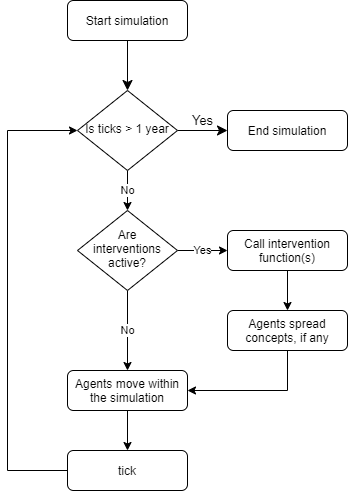
\includegraphics[width = 0.5\textwidth]{flow.png}
\caption{Flowchart showing the progression of the simulation.}
\end{figure}

\subsection{Decision process}
Thieves and Police take decisions with the objective of maximising their reward with a values-based learning algorithm, namely Q-Learning \cite{q1992} - Figure 4.2 shows the steps involved. Bicycles are generally in the same place during weekdays, which is why reinforcement learning was considered. Reinforcement learning is concerned with learning control policies where agents interact with an environment that is unknown to the agents \cite{qlearning}. This type of learning is widely used in the real world, for example with traffic light controls and in games where algorithms are used to solve games. \par 

\begin{figure}[h]
\centering
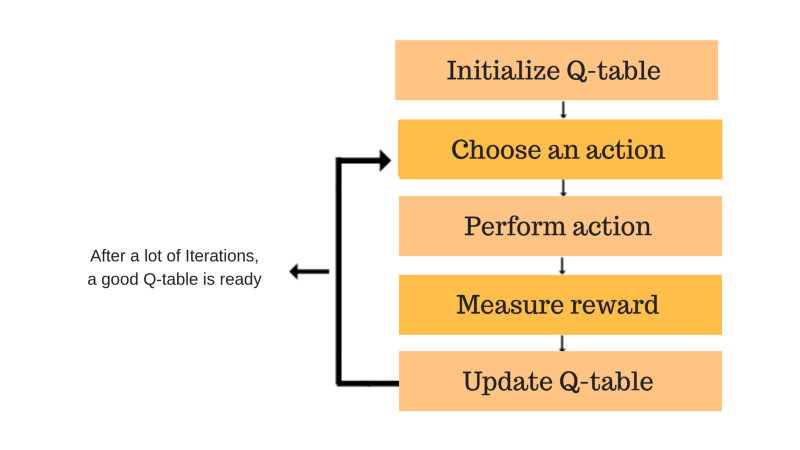
\includegraphics[width = 0.8\textwidth]{qlearningflow.png}
\caption{Each box shows one step of the algorithm. \cite{freecodecamp}}
\end{figure}

A Q-table is used to calculate the maximum expected future reward for actions at each state giving the best action at each state over time. The Q-function: \[Q(s,a) \leftarrow Q(s,a) + \alpha \cdot (r + \gamma \cdot max(Q(s',a')) - Q(s,a)) \]
\parindent \parindent Where:
\begin{itemize}
\item Q(s,a) is the Q value,
\item $\alpha$ is the learning rate,
\item r is the reward for taking an action in a state,
\item $\gamma$ is the discount factor,
\item max(Q(s',a')) is the maximum expected future reward.
\end{itemize}
The Q function is used to learn each value of the Q-table. Values are initialized to zero to begin with and are updated after an episode, the table acts like a reference table for agents to choose the best action based on q-value. An agent can interact with the environment in 2 ways, they can either exploit or explore. With the exploiting interaction the agent uses the Q-table as a reference and views all the possible actions for a state, the agent then chooses the action that holds greatest value of those possible actions- uses all information available to make a decision. The latter interaction, exploring, selects actions at random. This type of interaction allows the agent to discover new states that may not have been selected during the agent's exploitation process. \par

When a thief is in close proximity with another thief, the thief has the option to spread concepts to the other thief. If the concept is strong enough the agent can decide to accept the concept and alter their decision making accordingly, this may mean for example they view a bicycle of a perceived value to be too risky to steal or bicycles of low financial value are not worth the risk of being caught. \par

Bicycle agents in the model will primarily be in the same place daily as bicycles will be left near to the owner's place of work. Using the average working hours of workers in the City of London we can see that the majority of bicycles arrive into the environment between 800-1000 hours and leave between 1600-1800 hours.

\subsection{Interventions}
The interventions will be defined clearly in the interface. To apply an intervention to the simulation, the user must select the intervention(s) and run the setup procedure once again so the model is updated with the intervention(s).

\subsection{Output}
The simulation must output data that describes what occurred in the simulation run. At each tick a number of statistics will be reported:
\begin{itemize}
\item The tick number
\item The number of bicycles
\item The number of police officers
\item The number of thieves
\item The number of stolen bicycles
\end{itemize}
These will be stored in a comma-separate values file that is r....
\section{Interface design}
As the end users will predominantly be decision makers within Police forces, the interface will be as simple as possible. Because of this, the model is constructed in the NetLogo environment and this will be how users interact with the model. Since NetLogo is designed to be accessible to all types of computer users- from advanced programmers to those with few programming skills- users will easily be able to try out the model and design possible interventions and perhaps in the future model new possible interventions. \par

Although there will be default values for the parameters already, the first step of model setup is to select the model parameters which are available using sliders. This makes it possible to alter the population size, the number of agents and the number of each agent. The user prepares the model to run the simulation by pressing the Setup button. When the Setup button is pressed, it calls the \textit{setup} procedure from the model's source code. By running the \textit{setup} procedure, a map of the modelled area and the agents will begin to load based on the model parameters. If the user changes the value of a parameter after model setup, it is mandatory to run the setup procedure once again to echo the new values for the model parameters. \par

The model starts and runs by pressing the Go button, this is known as a forever button in Netlogo, since NetLogo continues to loop the \textit{go} command block until a certain criteria is reached which stops the model. Hence, users are only required to click Setup followed by Go to run the simulation.  \par

\chapter{Implementation}
As previously specified, the model will be implemented within the NetLogo environment which utilises its own language of the same name, NetLogo. NetLogo was chosen purely because of the software's relative ease of use for users who may not have prior programming experience, lowering the barrier of entry for those that would benefit from the model.  \par

An iterative approach was taken in the development of the model with successive versions improving upon the preceding version.

\section{Version 1}
The first version of the model was implemented with a focus towards agents and their movements within the environment whilst omitting interventions. Within the GUI the use of buttons in the model allows the model to be used by users with little or no programming experience. For users who have some experience with programming, they are able to enter commands in the command center which acts as NetLogo's command line. \par

\subsubsection{Setup procedure}
The \textit{Setup} procedure, which is initiated once the setup button has been clicked in the interface tab, sets the agents in the model, this being bikes, thieves and police. This is what is known as a \emph{once} button in NetLogo, the instructions associated with the button is executed once at the click of the button.\par

Setup starts by clearing all variables, turtles, patches, plots and drawings. This clears the whole model so that a new simulation can begin with nothing pre-set. The tick counter is reset back to zero allowing the model to completely restart from time zero and to update all plots accordingly. \par

Next, we create the agents that will populate the environment. The environment at this early stage in development will be a simple grid structure with no environmental features. Bicycles, thieves and police officer agents are added to the model with a ratio of 85:10:5 respectively. To make it clear which turtles are which in the model, turtles are given shapes. Bicycles are aptly defined as bicycles with a green bicycle representing a bicycle that is still in the possession of the owner and a red bicycle representing a stolen bicycle. Thieves are the red characters in the model and police are the blue characters in the model. \par

Bicycles have a random desirability and security between 0 and 1 assigned to them from the start of their agent creation. The desirability value is a fixed value depending on the value of the bicycle and the security value may change depending on interactions during the simulation which affects the way the bicycle is secured. Thieves enter the world with a crime-probability value, this is given randomly but can change throughout the simulation. 

After the agents have been created, the model is ready. To note, agents begin the simulation with no knowledge about the environment and are in an exploration phase where they randomly explore the environment. Over the duration of the simulation the agent would build up knowledge from reaching grid cells and be successful with their goals.  

\subsubsection{Go procedure}
The \textit{Go} procedure is what makes the model start running. This is where agent interaction is controlled. First we deal with the interaction between thieves and bicycles, bicycles are stationary for the majority of their lives and thieves travel within the environment scouting bicycles to thieve. Each thief enters the environment with a crime probability, that is the likelihood that they commit a theft, if the thief's crime probability is greater than the threshold for theft and the thief is in a patch with a bicycle that is poorly secured with a low security value, the bicycle will be stolen. All agents are able to navigate freely within the world, this includes police agents who patrol the world in search of thieves.\par

\paragraph{}
The model has been set with each tick representing one day, 24 hours. With the agents interacting as they should we can now add more functions to the model.

%agents do not leave the model at any time
%agents are in the environment at all times
%one week is one tick \par

\section{Version 2}
%added map, talk about patches, agents limited to roads
%variable number of agents
%q learning algorithm
The second version was a continuation of the first version but with a focus on the interface and the decision making of agents. \par

Agents are now able to leave the environment forever for example if a thief feels the risk in the location is too great and stealing bicycles is too risky and they choose to thieve elsewhere or due to policing they decide to no longer thieve. 

\subsubsection{Interface}
Instead of a fixed number of agents in the previous version, the user is now able to change the population size of the model and the ratio of the individual agents via sliders - the sliders are a quick way to change variables. With this, users are able to compare results of the simulation easily without recoding the procedure every time. 

The interface now also includes a map of the modelled environment which is initiated in the \textit{setup} procedure, the environment being a small area of the City of London. The area is 1265 x 429 which gives a total of 542,685 patches. Obviously not all of these patches will be available for the agents, the patch could be a building or a road. \par

The previous version of software featured ticks that were equivalent to one 24 hour period of time. Whilst the simulation can be slowed down manually in NetLogo it was clear than one tick was too quick and the model simulated time too quickly. As a result, the time of 1 tick was changed to one hour- meaning each tick was equivalent to one hour of time, 24 ticks models 1 day. As previously said the unique nature of the City of London whereby population drastically declines on weekends and public holidays, the model will only model 261 calendar days. With each tick representing 1 hour of a day, the model will run for 6264 ticks.

\subsubsection{Agent decision making}
In the previous version, agents roamed around the world looking for bicycles with no set plan- this is where q-learning is involved. For each type of agent, patches have different q-values for example, a thief with the next patch being a bicycle will have a higher q-value than a police agent. This is because the value that is gained from taking that step is greater for a thief than other agents. For thieves a patch that contains another thief has the q-value of 0, given that they have nothing to gain, a q-value of 10 if the patch contains a bicycle and a q-value of -10 if the patch contains a police officer. This is similar for police agents, a patch that contains a thief has the q-value of 10, a q-value of -10 for a patch with another police agent and a q-value of 2 for a patch containing a bicycle. 

With the patches now having q-values dependent upon the agent that is looking at the patches we can now finalise the q-learning algorithm by computing the q-values looking at north, east, south and west to decide upon which patch to move to next. We use the q function as stated in 4.2.2 to calculate the q-value for all four possible directions and the greatest q-value is then taken as the optimal action from that patch. \par

From quick testing, it was apparent that using variable rates in regards to the learning rate and discount factor of agents within the q-learning caused poor performance and fluctuating results. As a result, moving forwards it was decided that fixed constants would be used.

\subsubsection{Interventions}
For simplicity for the user, possible interventions are activated with the use of buttons within the interface. The user simply activates the intervention and set the model up ready for simulation.

\subparagraph{Police give advice to thieves} 
\paragraph{}
Police agents give advice to suspected thieves to stop stealing bicycles. Agents choose whether or not they want to listen to the advice given and their crime probability is reduced accordingly if they do listen. If the agent's crime probability reaches the low threshold, the agent then leaves the environment to either steal bicycle's elsewhere where they feel it is safer for them to do so or they stop stealing altogether. 

\subparagraph{Police offer bicycle locking advice}
\paragraph{}
Whilst patrolling the environment, police agents offer advice on how to lock bicycles making them more secure whilst left unattended. This can be done without the owner being present through the attachment of leaflets to bicycles. Once again, agents can decide whether or not to take this advice on board but if the agent does there bicycle will have a higher security- which should in theory make it more difficult for thieves to steal and in turn deterring thieves to steal the bicycle.

\subparagraph{Encourage bicycle marking}
\paragraph{}
By having a bicycle security marked if a thief was caught with a registered bicycle that is reported stolen the thief can be arrested and the bicycle can be returned to the rightful owner. Due to the threat of arrest if caught with a marked bicycle, this acts as a visible deterrent to possible thieves. The bicycle has a lower desirability to thieves due to the increased risk. This can be done similarly to offering locking advice through leafleting and bicycle agents interacting with one another.

\subparagraph{Advise the removal of expensive parts from bicycles when left unattended}
\paragraph{}
Bicycles frequently have parts to them that make them particularly attractive to thieves for example saddle and accessories. By removing these parts when the bicycle is left unattended, the value of the bicycle is reduced and the bicycle may be seen as less desirable in the eyes of a thief. In the case of removing a saddle from a bicycle, this makes it more difficult for the thief to transport the stolen good if they were planning on door-to-door transport to sell. 

\section{Version 3}
The completion of the previous version, version 2, marked the completion of core functionality of the model however improvements can still be made. The previous versions were too slow to be used practically, taking a considerable amount of time to complete the simulation even in the fastest setting in NetLogo. The source code for the simulation was profiled to identify the slow parts and bottlenecks in the simulation were discovered. 

\subsubsection{Performance improvements}
When an agent is in close proximity to another agent, instead of just interacting with that said agent the agent would instead interact with all of the same agents within the environment to then check who was nearby and in a close distance. This was rectified by limiting the radius in which an agent can interact. 

It was also clear that the agent decision making process as set out in Section 4.2.2 was slow. There was an issue whereby there were too many agents on one grid space and new agents that wanted to enter that grid space were forced to wait for that grid space to become available. One grid space in the environment is the equivalent to roughly a few square meters, in the real-world bicycles and people are not that physically close and so by limiting the amount of agents per grid space agents were able to move quicker by being forced to go elsewhere if there choice of grid space is unavailable. \par

In previous versions, bicycles would enter the environment whenever they wished- this is unrealistic, with bicycles sometimes entering the environment at the equivalent to 0300 hours. The peak time of travel within the City of London is between 0800-0930 hours in the morning and 1630-1900 hours in the evening. To account for this, the majority of bicycles are set to enter and leave between those times in the equivalent time in ticks. \par

There were clear bottlenecks in the interventions, this was down to interventions not being targeted to agents and instead targeted to all agent types in the model. This was easily rectified by only calling the needed procedures when certain conditions were met, so only suspected thieves would receive advice from police agents and bicycles do not.
\section{Testing}
By choosing to follow an agile development cycle, testing of functionalities in the model were done iteratively with each subsequent version and little testing was required to ensure that the software was performing as required. Nonetheless time was required to test individual variables in the model, as minor adjustments of these numerical values would cause severe changes in agent behaviour. There was a great deal of trial and error testing involved in seeking default values for the model so that the model would produce a realistic and balanced simulation.   

\chapter{Professional Issues}
Throughout the implementation of the project, great effort was taken to abide by the British Computer Society (BCS) Code of Conduct \& Code of Good Practice. Any Open-Source code or libraries used in the project has been made explicitly clear. This project consists of my own work and Open-Source code and where Open-Source code has been used, it has been modified to suit the requirements of the project. \par

It is important to note that this project does not act as an accurate simulation of bicycle theft in real life. Due to the under-reporting of bicycle thefts, it is impossible to accurately validate this model. The intended purpose of this model is to show how thieves \textit{may} be deterred in carrying out bicycle theft. 

\chapter{Results}
Creating a model that would be able to simulate possible interventions to judge viability was an important part of this project. This following section will outline experiments performed using the model to demonstrate the model's utility as a tool and express the results from said experiments. \par

Experimentation can be split into two distinct types with this model, with the first being model experimentation. This type of experimentation is used to explore changes in the simulation by changing the way the agents work, focussing upon the model behaviour rather than trying to replicate real-world scenarios. By changing variables such as the learning and discount rate it is possible to affect the performance of the agents. Testing this would be useful in trying to make the model behave similarly to the real world and using it to replicate other real world phenomena. \par

The second type of experimentation will focus on the interventions set out with the use of scenario experimentation, this will be similar to what the end user would use the model for. The end user would not be concerned with the specifics of the software, for example how each agent works, how each agent interacts within the model and how they are initiated in the model, but instead focus on the testing variables and attempting to apply the model to the real world.

\section{Testing parameters}
To ensure consistency of results, elements that are used in testing that are consistent throughout are explicitly defined. They are as follows:

\begin{table}[]
\begin{tabular}{|l|l|lll}
\cline{1-2}
Parameter & Value \\ \cline{1-2}
Population size & 12000  \\ \cline{1-2}
Ratio of thieves & 0.01 \\ \cline{1-2}
Ratio of bicycles & 0.25  \\ \cline{1-2}
Ratio of police & 0.10 \\ \cline{1-2}
Minimum agent learning rate & 0.1 \\ \cline{1-2}
Maximum agent learning rate & 0.9 \\ \cline{1-2}
Agent discount factor & 0.8 \\ \cline{1-2}
\end{tabular}
\end{table}

The values above were decided through development of new functionalities. The result of these values produces a balanced behaviour in agents. \par

There is only a clear 'win condition' for thief agents within the model, it is in their best interest to steal as many bicycles as possible. Due to the nature of interventions model runs simply conclude after a fixed number of ticks as is already done in the model, 6264 ticks was decided upon after the exclusion of weekends and public holidays where footfall in the real-life environment drastically declines. \par

There is only one value that is important in the model and that is the total number of bicycles that are stolen over the duration of the simulation. Using this value we are able to see how 'well' agents performed and evaluate the effectiveness of interventions. The higher the value, the 'better' thieves are doing- this value shows the success of both thieves and police whilst also looking at changes within bicycles as thieves are in direct competition with all other agents.  

\section{Model experiments}
\subsection{Considering the learning rate of agents}
Learning rate determines the speed at which agents are able to take on new information, this usually takes the form of a constant or a variable. The following experiment aims to examine how changing the learning rate affects the number of bicycles stolen. 

\subsubsection{Learning rate with no interventions}
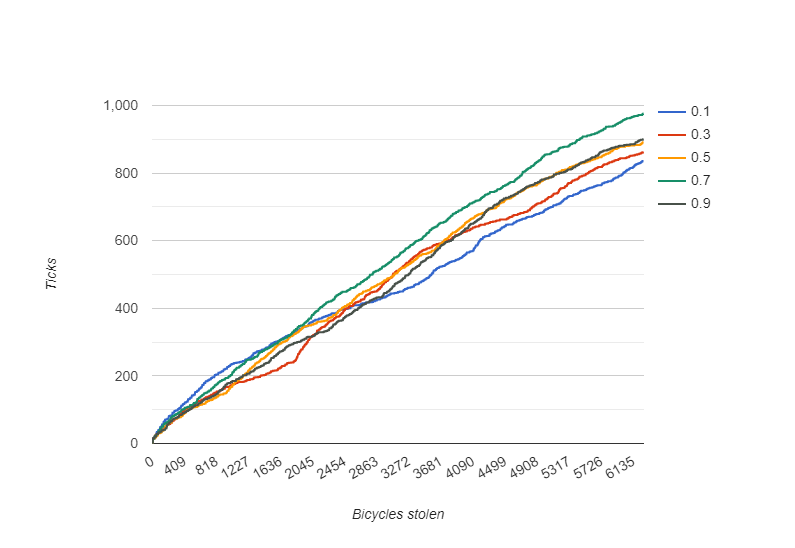
\includegraphics[width = 1\textwidth]{learning.png}

Whilst not substantial, there is an apparent difference in agent effectiveness when using differing learning rates. With no interventions present the agents have the greatest opportunity to steal bicycles. A constant low learning rate in the agents performed as expected and unsurprisingly the experiment with a learning rate of 0.1 gave the worst results. Agents utilising lower learning rates were less effective at stealing bicycles than compared with greater learning rates suggesting a low rate is not preferable. The higher rate of 0.9 is more effective however peaks at certain points and fluctuates throughout, this is expected as with high learning rates that are close to 1 the agents ignore all prior knowledge and solely consider the most recent information via exploration. The results show that a learning rate between 0.7 and 0.9 is most optimal with the greatest performance in theft, this value acts as a compromise between a high value and a consistent value. 

\subsubsection{Learning rate with interventions}
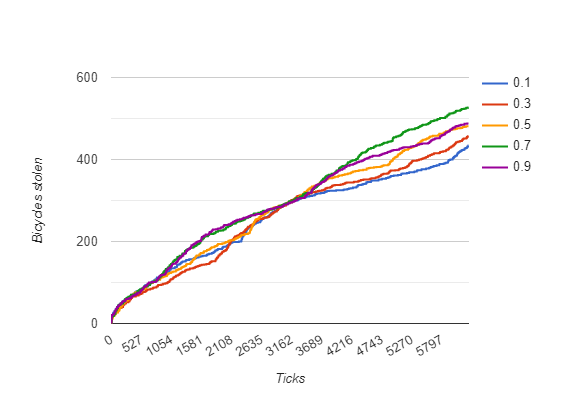
\includegraphics[width = 1\textwidth]{learningwithintervention.png}

With the addition of interventions, the difference in agent effectiveness is made more clear. This experiment uses all of the possible interventions available in the model. As before, the low learning rate returned the worst results and the trend is a higher learning rate delivered greater results. Once again there reaches a point where a high learning rate no longer delivers and results start to suffer, the results shown here reinforces the results seen previously. A learning rate of 0.9 initially performs better than the learning rate of 0.7 but is less favourable as we reach the latter stages of the run. We can confidently say that the model is most optimal with a learning rate between 0.7 and 0.9.

\subsection{Intervention experimentation}
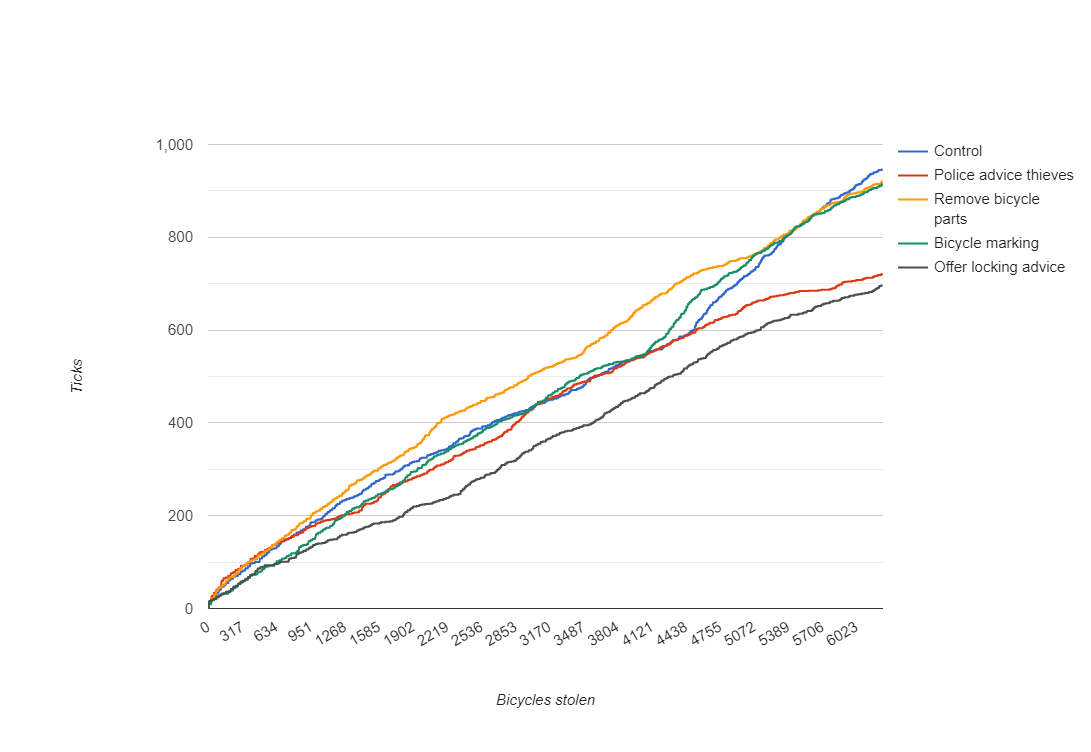
\includegraphics[width = 1\textwidth]{all.png}

The above graph shows results with interventions present. There are varying results with the interventions with some interventions showing promise whilst others not so much. A control is included which shows theft with no interventions present and is used as a comparison against results with interventions present. \par

As it can clearly be seen in the graph, removing bicycle parts from a bicycle when leaving it unattended does little to deter theft and at points even attracts thieves to steal it. This may be due to the fact that as there are missing parts, thieves may think that the bicycle is abandoned anyway and stealing it when it has been abandoned is seen as less risky. Another intervention which is worth noting is bicycle marking. In theory by security marking a bicycle, thieves should be deterred from stealing them as if they are caught with them and they have been reported as stolen it is an offence. The results show that bicycle marking makes little difference by itself but it is also worth noting that if the bicycle is found eventually, there is a chance that the bicycle can be recovered and returned to its owner. \par

Of all the interventions, offering locking advice shows the most promise and with that a considerable drop in thefts. By offering locking advice bicycles can be left more secure whilst unattended, whilst the bicycle can still be stolen by a determined thief there is more risk on the thief agent stealing a bicycle that is secured well.  More time will need to be spent with said bicycle to free it from its locked state which may arouse suspicion of nearby people in the real-world. When observing the model visually, the thief agents could be seen going past secure bicycles and instead targeting bicycles that are less secure.
\subsubsection{Combination of interventions}
For interventions to make an impact, it would be best to use a combination of interventions. 

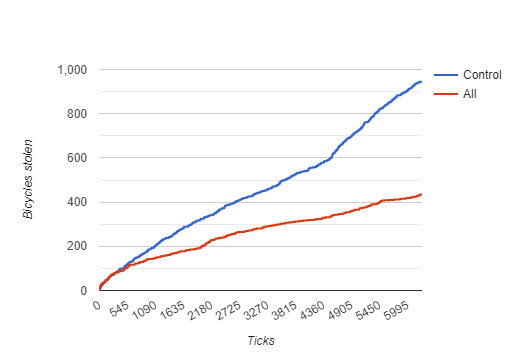
\includegraphics[width = 1\textwidth]{inteventionvsno.png}
The blue line shows bicycle theft with no interventions present whereas the red line shows all interventions being used. In an ideal world where all possible interventions could be implemented the results are positive and there is a clear drop in the projected bicycles being stolen as a result of thieves being deterred to thieve in the modelled location and also thieves deciding that the risk no longer outweighs the reward. This is wholly unrealistic given the many interventions that are being modelled. The modelled simulation includes police advising suspected thieves against thieving, encourage the removal of expensive bicycle parts, encourage bicycle security marking and offering secure locking advice.


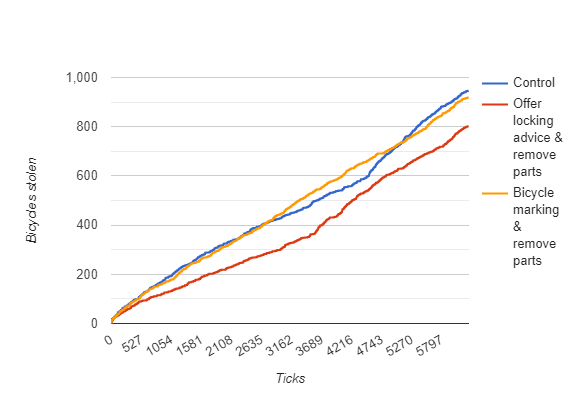
\includegraphics[width = 1\textwidth]{lockingadvice.png}
This experiment followed on from the experiment with individual interventions. With the combination of interventions we are able to notice how one intervention may work well with other interventions. From the graph we can see the control, which is the simulation with no interventions present. Encouraging bicycle security marking and encouraging owners to remove expensive parts from their bicycles makes little difference to overall theft. From this we are able to conclude that by removing bicycle parts it fails to act as a deterrent and should not be used as an intervention moving forwards. Offering locking advice is a more suitable intervention with a clear decrease in thefts, this may be due to the increase in bicycles being locked securely which makes it more difficult for thieves to steal.

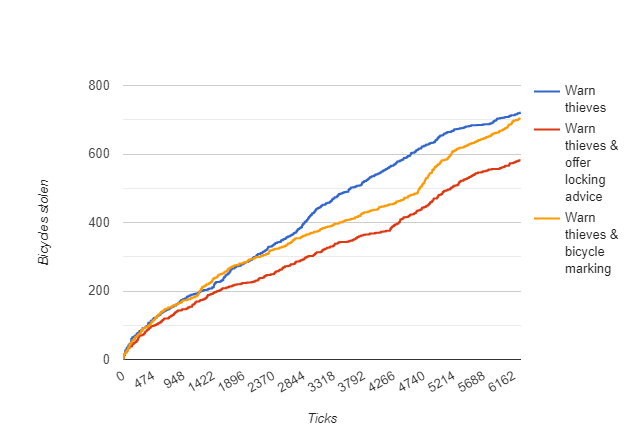
\includegraphics[width = 1\textwidth]{warnall.png}
Police giving advice to suspected thieves to stop stealing bicycles was discovered to be effective in experimentation. This may be due to the fact that thieves are aware of the fact that their actions have been noticed and that there may be a greater risk in the future of being caught whilst committing a crime, in effect increasing the risk of committing bicycle theft. \par

When experimenting the warning thieves intervention with other possible interventions, it was found that when combined with encouraging bicycle security marking thefts there was little effect overall. It is clear that warning thieves against stealing bicycles is effective in some form but bicycle marking makes little difference in deterring thieves from stealing bicycles. \par

Offering advice on how to securely lock bicycles shows some promise when in combination with warning thieves, there is a decrease in thefts when compared with just offering locking advice by itself. 

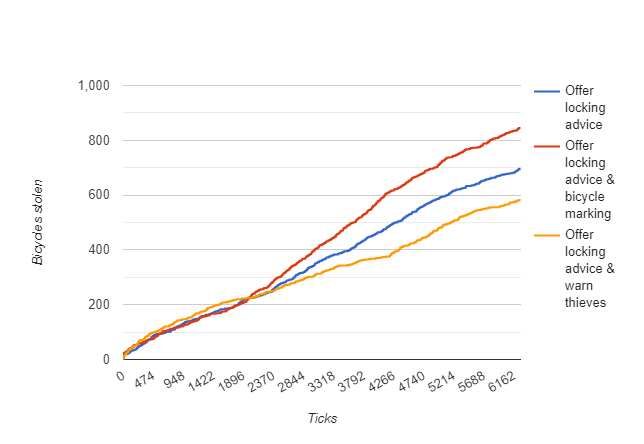
\includegraphics[width = 1\textwidth]{lockall.png}
From the initial experiment it was found that offering locking advice on how best to secure a bicycle resulted in the greatest drop in thefts. This experiment focused on the potential implementation of other interventions alongside it. In earlier experiments we found that bicycle marking offered little in the act of deterring thefts but instead aided the return of bicycles if successfully recovered. In combination with bicycle security marking and offering bicycle locking advice, results were surprisingly poor. Over time, thefts of bicycles after the combination of interventions were made actually suffered than compared with just offering locking advice. We can speculate that this could be down to the fact that the bicycle is security marked it is perceived to be secure and that there is no need to securely lock it. \par

As we found earlier the best reduction in thefts came from offering bicycle locking advice and police warning suspected thieves individually. Combining these two interventions showed the most promise with a drastic reduction in bicycle thefts. With bicycles more securely locked when left unattended and thieves being made aware of the risks of being caught with stolen bicycles, the risk vs reward is changed significantly. Whilst the reward of the bicycle remains the same, the risk is adversely changed for the greater.
\chapter{Evaluation}
\section{Requirements}
To ensure that the developed software is complete, it was evaluated against the earlier described requirements in Section 3.2. 

\subsection{Simulation requirements}
\begin{itemize}
	\item \textbf{The simulation must run for at least 1 year.} Due to the unique nature of the City of London it was decided that it best to only model 261 calendar days.
	\item \textbf{Agents come and go throughout the day.} At each time tick agents in the model are free to move within or even leave the environment if they so do wish.
	\item \textbf{Due to the uniqueness of the City of London whereby the resident population is 7375 with a 56 fold increase in workday population, according to data from the 2011 Census \cite{ons2011}, the simulation will ignore weekends and holidays where the footfall is dramatically reduced.} As explained above, the model ignores weekends and holidays and models 261 calendar days.
	\item \textbf{The simulation must allow the user to call intervention functions to manipulate the simulation world (agents and environment).} The user is able to call interventions by simply selecting the intervention buttons in the interface.
	\item \textbf{The simulation must return statistics at the end.} Statistics can be seen in the monitors in the interface, graphs can be exported to see more in-depth statistics.
\end{itemize}

\subsection{Agent requirements}
\begin{itemize}
\item \textbf{Agents in the simulation must be free to come and go.} Each agent in the model has its own decision making and is able to move within the environment or to leave altogether.
\item \textbf{Agents must observe the environment and react to any changes that occur accordingly.} As described in the design chapter, agents have a utility function whereby they are able to observe the environment around them and it is this surrounding environment that affects decision making.
\item \textbf{A bicycle must either be in a locked or stolen state.} Each bicycle agent can either hold the variable whereby it is locked or a state where it is stolen.
\item \textbf{A bicycle must be able to hold concepts.} Each bicycle has a security variable attached to them, this variable can be affected by the adoption of concepts from other bicycles.
\item \textbf{A bicycle must be able to spread concepts to other bicycles.} When a bicycle is within close proximity to another bicycle they are able to spread and adopt concepts.
\item \textbf{Thieves must either be active or inactive.} Each thief can either be in state where they are active or inactive.
\item \textbf{Thieves are able to steal bicycles.} For thief agents it is their goal in the model to steal bicycles, it can be said that if they do not steal a bicycle they have not succeeded.
\item \textbf{Thieves attempt to avoid Police.} As described in the design, the agent has a utility function that it uses to decide where to go, if they are near a Police agent they will attempt to take a different route.
\item \textbf{A thief must be able to spread concepts to other thieves.}When a thief is within close proximity to another thief they are able to spread and adopt concepts.
\item \textbf{Police must either be active or inactive.} Each police agent can either be in state where they are active or inactive.
\item \textbf{Police must be able to spread concepts to both bicycles and thieves.}When a police agent is within close proximity to suspected thieves or bicycles they are able to spread concepts.
\end{itemize}

\subsection{Environment requirements}
\begin{itemize}
	\item \textbf{The environment must represent a real-world physical area within London.} With the use of a PNG image, the model models an area of the City of London.
	\item \textbf{The environment must support the definition of properties and through-way.} The PNG image as discussed above sets out the roads and buildings with the use of different colours. Within the model itself, agent movement is restricted to areas that are seen as roads or pavements with the use of patches. Areas that are deemed as buildings from the PNG through the colour of the patch are not accessible by agents.
	\item \textbf{The number of agents within the environment must be adaptable by the user.} The user is able to adjust the number of agents by changing the overall population within the environment or individually change the ratio of each agent.
	\item \textbf{Bicycle and thief agents must not be able to enter buildings that will be clearly defined in the simulation.} Through the use of the coloured PNG image of the area, agents are restricted to only the public roads and footways.
	\item \textbf{The environment should be as realistic as possible.} The environment is a small area within the City of London.
\end{itemize}

\subsection{NetLogo requirements}
\begin{itemize}
	\item \textbf{The user must be able to setup, run and stop the model.} Through the use of buttons within the NetLogo interface, the user is able to simply setup, run and stop the model.
	\item \textbf{The simulation within NetLogo must create some agents within the environment and interventions to be used in the model.} At the setup stage of the simulation, agents propagate in the model, possible interventions are pre-set and can be used at a click of a button.
	\item \textbf{NetLogo must run the simulation.} This can be simply achieved by setting up the model and pressing \textit{Go}.
	\item \textbf{NetLogo must offer variable changes.} Changes to variables can be made with the use of the sliders. If the user wishes to change the learning rate or discount rate in the agent decision making this can be done by changing the variables in the source code.
	\item \textbf{NetLogo must create some graphs to describe the simulation run.} A graph is outputted to the user as the simulation progresses but due to NetLogo's restrictive nature this will need to be exported to a CSV so that more in-depth analysis can take place.
\end{itemize}

\section{Experimentation}
The results chapter of this report shows how the software could be used in real-world application and showed promising results that were interesting and could be explained intuitively. With the results from the experiments more interventions can be be tried with the model and greater combinations to find the most optimal solution.

\chapter{Conclusion}

\section{Conclusion}
This project relies on behaviours of agents and it is clear greater research needs to be done to understand the psychology of a criminal so that modelling their behaviour can be more accurate and reliable. \par

The project aimed to create a piece of software that modelled bicycle theft in London that could be easily used by someone with little technical knowledge. In this way it can be said that the project was quite successful, however using NetLogo was rather restrictive at times and if another system was used implementation could have been made simpler and agent behaviour and interactions could have been made more complex to simulate it similarly to real-life.

\section{Future Work}
Many improvements and additions can be implemented in future iterations of the model. With the ease of additions in NetLogo, this would be relatively easy if necessary. \par

When thinking about the environment, a clear improvement would be to add street-level features like CCTV and lighting to the model that would affect agent decision making. This will obviously take a large amount of time to accurately map the locations of these environmental features however analysing the influence of readily available public safety elements would be useful. \par

Another major improvement that could be made would be the addition of weather modifiers, this would allow the user to be able to simulate how weather affects agent behaviour. Perhaps fewer bicycles being on the streets in addition to poor weather detract thieves from going to an area to steal. \par

Agent-based modelling is a very useful tool and there are many opportunities to develop this project further to achieve fascinating results.
\cleardoublepage
\addcontentsline{toc}{chapter}{Bibliography}
\printbibliography

\appendix
\chapter{User Guide}
\section{Environment setup}
\subsection{Installing NetLogo}
In order to run the simulation you must first install NetLogo, the simulation was developed in Version 6.1.1 (September 2019) and may not be backwards compatible with earlier versions of NetLogo. To do this visit https://ccl.northwestern.edu/netlogo/6.1.1/ and download the relevant application depending on your current operating system. 

\subsection{NetLogo }
\begin{itemize}
\item Interface tab : This is the main tab where the user interacts with the model and agents behaviour is visualised. It contains buttons, sliders, switches, monitors and plots.
\item Information tab: This contains information for the user on how to use the model.
\item Code tab: This contains all the source code.
\end{itemize}
\subsection{Running the simulation}
With NetLogo now installed, you are now able to go to the root folder of the simulation and open the nlogo file. Once opened, you will be presented with the main view in the centre and various buttons, sliders and monitors to the left of the main view as seen in figure A.1.

\begin{figure}
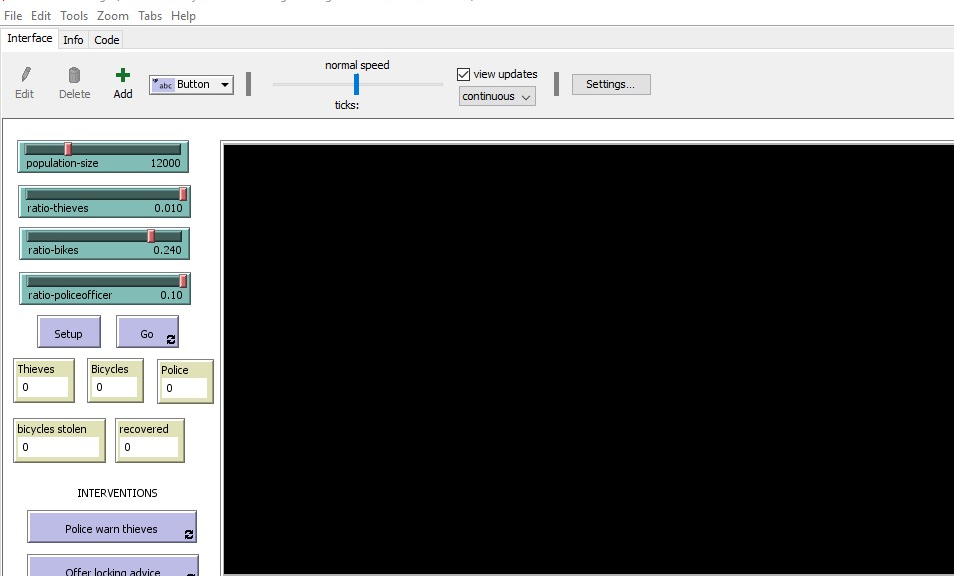
\includegraphics[scale = 0.4]{interface.png}
\caption{The NetLogo interface}
\end{figure}

The sliders allow you to change the population of the area that is being simulated and the ratio of each of the agents. The possible interventions are at the bottom, it is possible to run the simulation with no interventions, certain interventions or a combination of the interventions. Once that is decided click the Setup button to setup the model, agents will now appear in the main view as denoted by the respective characters in the simulation. If there are any changes to the interventions or the variables, the model needs to be setup again with the use of the Setup button. To run the simulation, click the the Go button- this will run the simulation for one calendar year in the respective number of ticks. To note, in the simulation one tick is equivalent to one hour of time. \par

The speed of the simulation can be changed using the speed slider in the upper toolbar, it is set at normal speed by default. It is important to ensure that the view updates box is applied, this ensures that updates can be seen visually in the interface. \par

With the model now setup, the interface should look like figure A.2. 

\begin{figure}
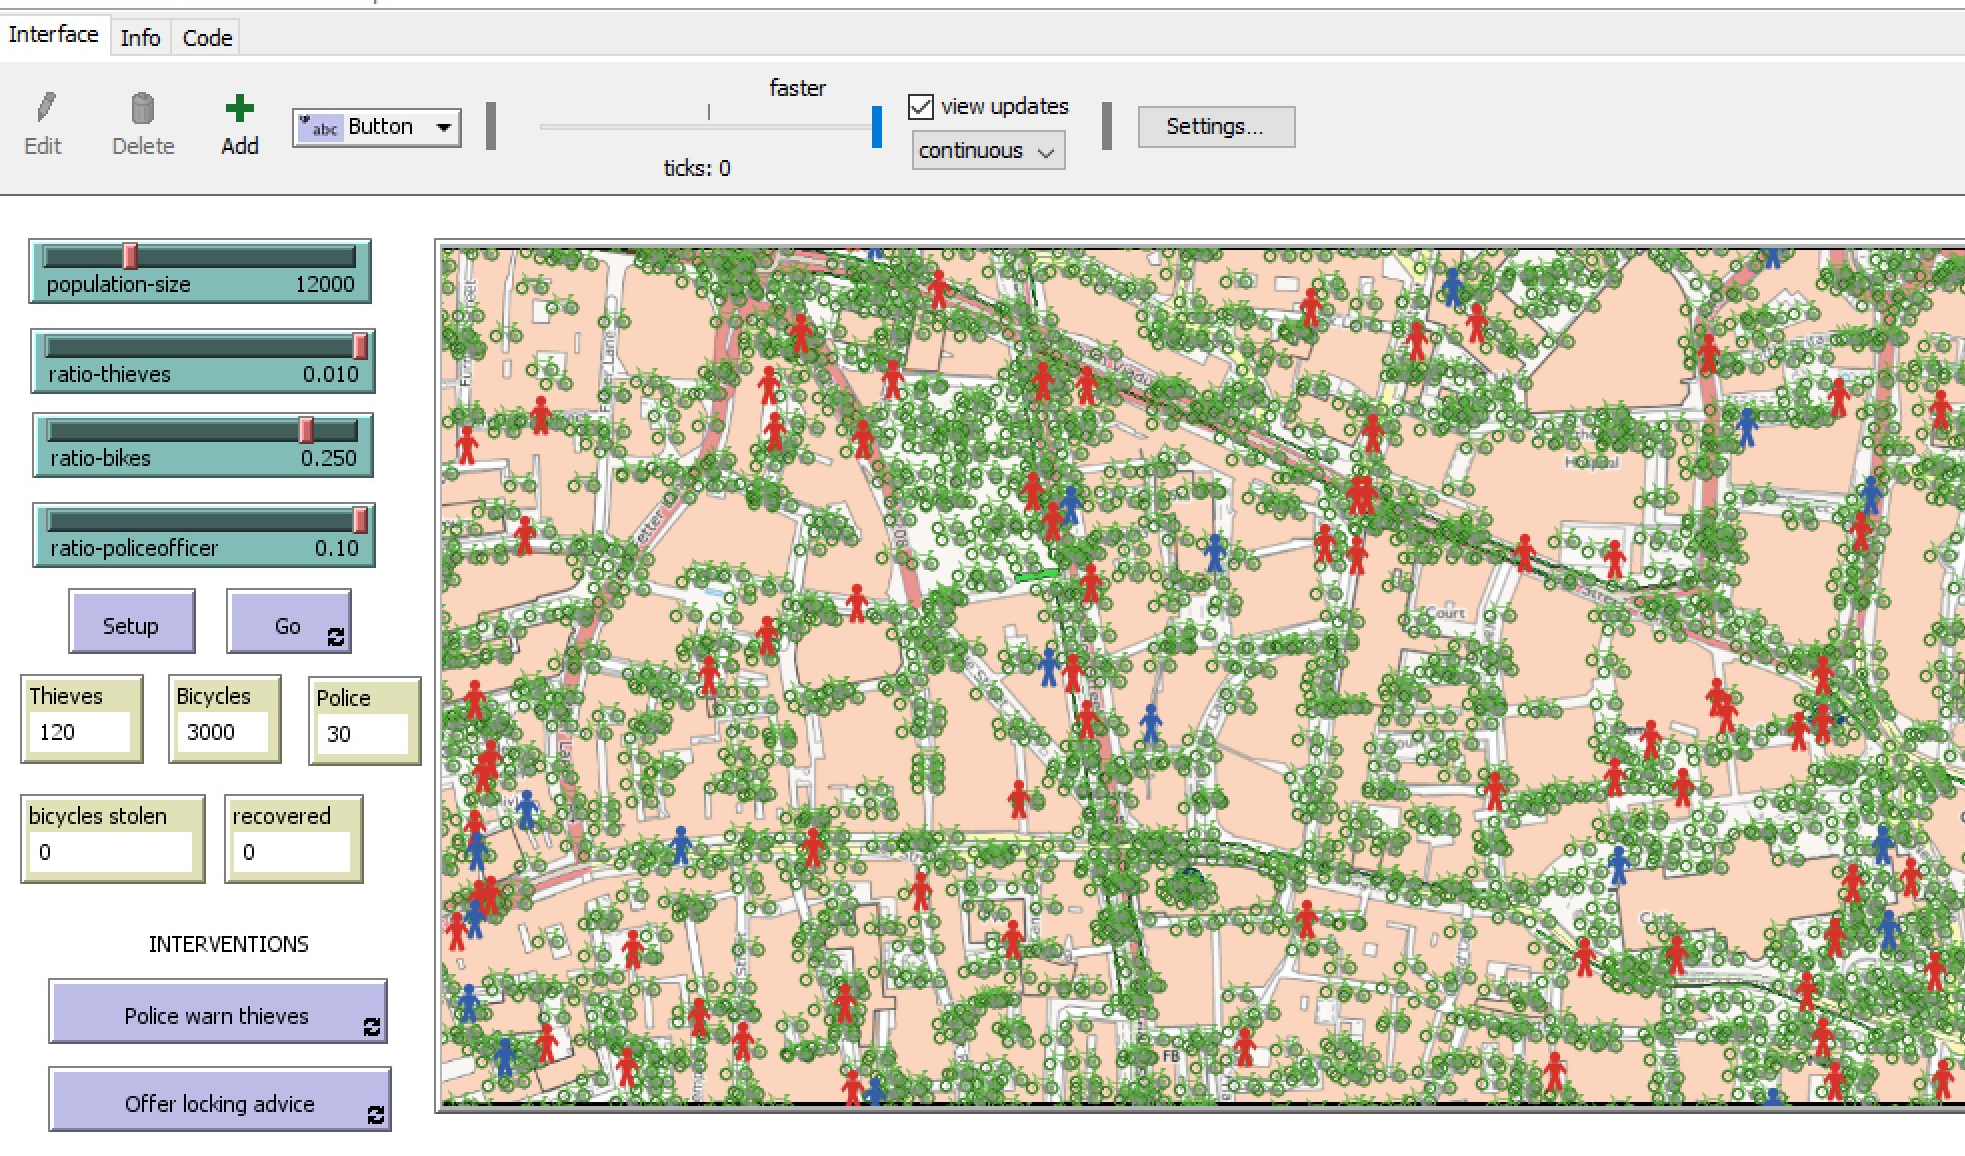
\includegraphics[scale = 0.4]{setup.png}
\caption{The NetLogo interface once setup has been completed}
\end{figure}

\chapter{Source Code}
\section{Avowal}
I verify that I am the sole author of all code, except for a minor section in the Q-learning in the decision making of agents whereby open-source code was modified. The author of the original code is Larry Lin and the code can be found on Modelling Commons \cite{larry}. This has been made explicitly clear.

\section{Source}
 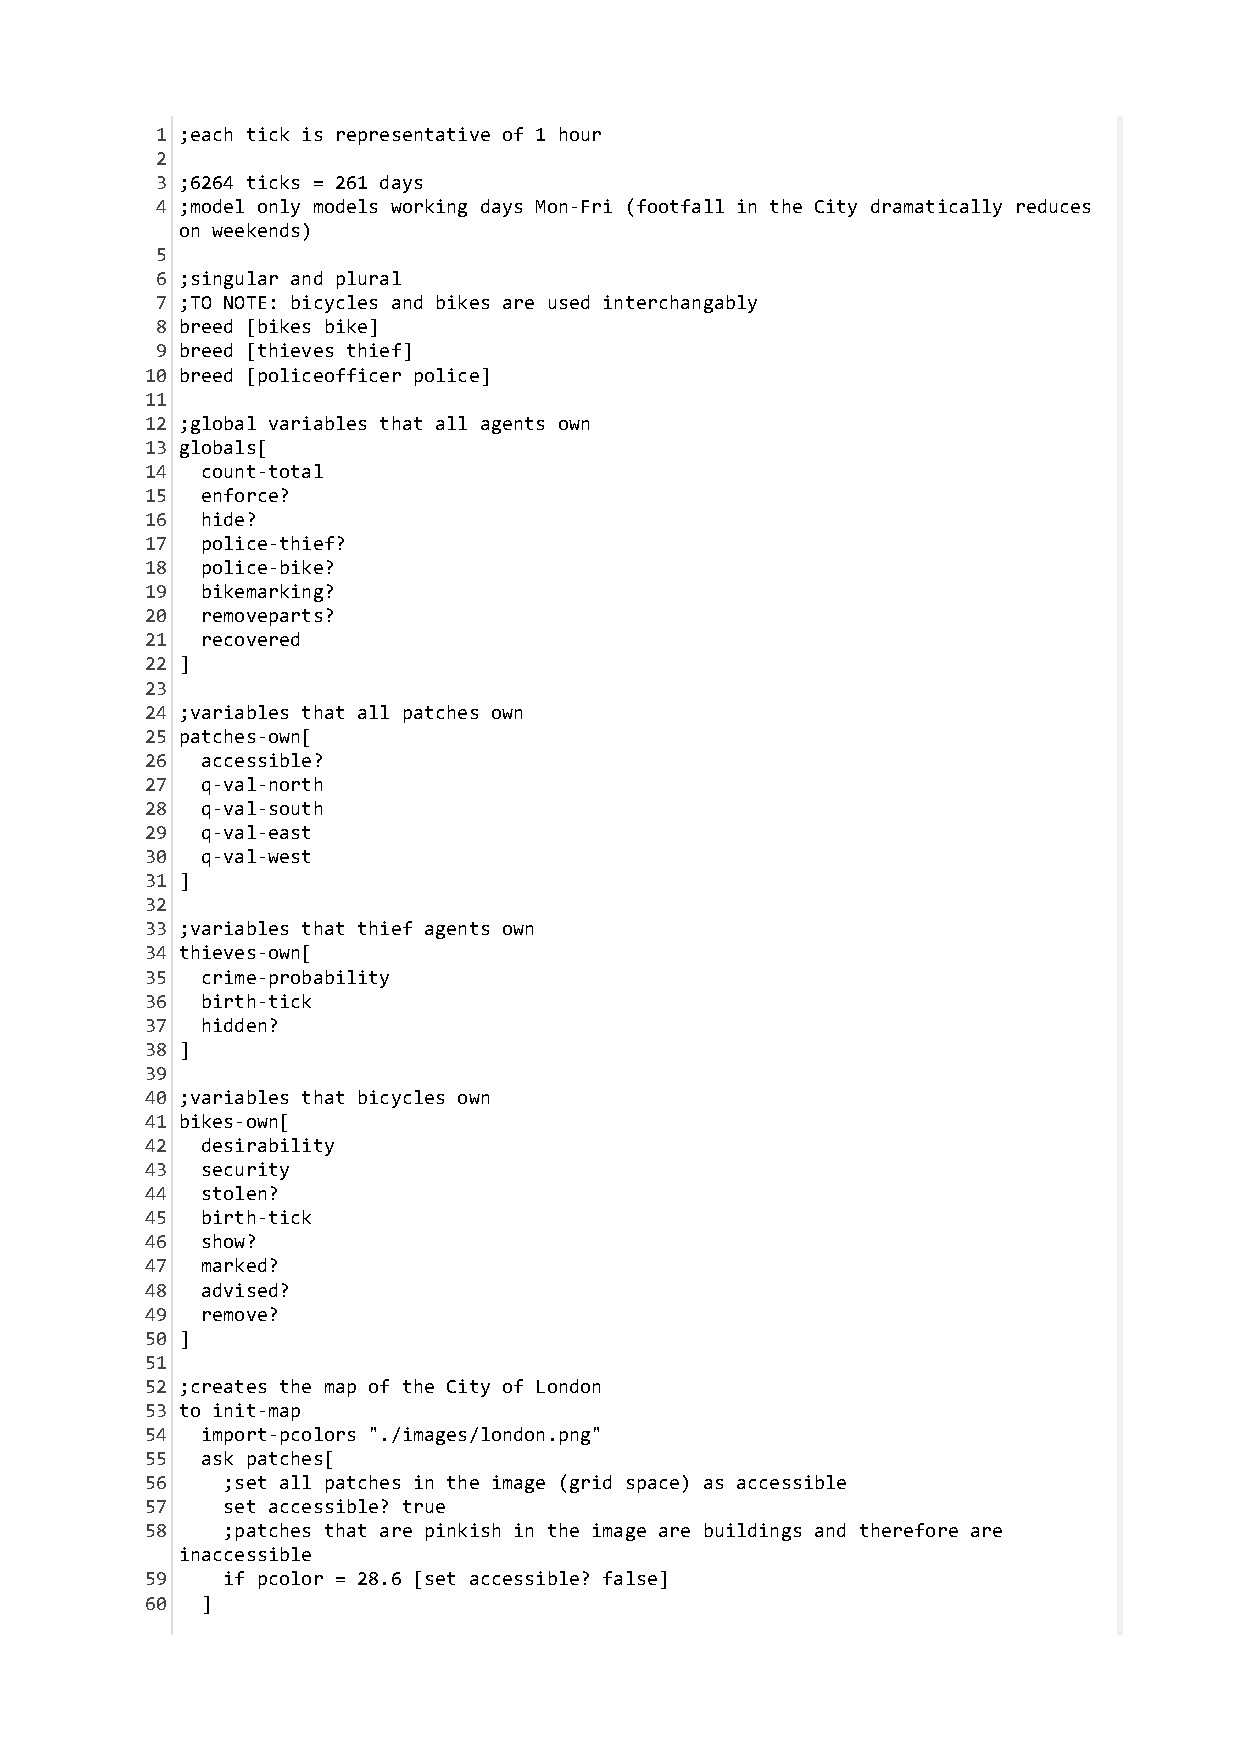
\includepdf[pages=1-19, pagecommand={}]{code.pdf}


\end{document}
